% Introduction

\pdfbookmark[1]{Introduction}{Introduction}

\chapter{Methodology}
\label{chap:methodology}

\begin{flushright}{\slshape    
If it disagrees with experiment, it's wrong.\\ 
In that simple statement is the key to Science.} \\ \medskip
--- Richard Feynman~\cite{Feynman:1965}
\end{flushright}


\bigskip


\section{The importance of being naive}
\label{sec:the_importance_of_being_naive}

\section{In defense of reductionism}
\label{sec:in_defense_of_reductionism}

In fact, we do not need to have a full theoretical description of the human mind
to say something about the actions of hundreds of thousands, a million of them.
In the same way we do not need string theory in order to explain the
functioning of living organisms.

Randomness is not to be understood as the opposite of rationality. Individuals
may as well make perfectly rational, predictable decisions, we would still have
to use a probabilistic approach. Particles are an extreme example of individuals
with a rational behaviour, yet we describe their collective behaviour with
statistical physics. Probabilities are not called for by the unpredictability of
one's behaviour, but rather by the particular type of information that is
important to us -- and that we can process.

What tells us that the world is not more complex than the picture drawn by
physical theories? That our best theories are only approximations that work a t
a certain scale, but are plain wrong at others? Everything around us, and the
history of physics itself. Reductionism does not imply renouncing to the world
in its entirity and its complexity. Reductionism is merely a recognition of our
limited capabilities, our possibility to grasp only the world tiny bit by tiny
bit, approximation after approximation. It is not absurb to reduce the amount of
information that is dealt with in theories, because this seems to be exactly how
we are cognitively programmed to function. If our brains were able to embrace
the world in all its details at once, one wouldn't need models, one would not
need theories, one wouldn't need science. Observation would be synonymous 
understanding.\\
History of Physics tends to prove to us that, in fact, all theories \emph{are}
effective theories -- in the sense that they are only true at a given scale. Too
aproximate when our measufing apparatus are able to probe nature more into
details. The analogy here is clear: we need more data, more specific data first
if we want to dig deeper into the reality of our societies, economies. We need
more than our own eyes, more than our ears. We need social, economical
telescopes.

\section{Quantitative stands for 'data'}
\label{sec:quantitative_stands_for_data_}

Richard Feynman's statement used as an epigraph in this chapter might be an
oversimplified, narrow view of what Science is and how it proceeds. It
nevertheless hits the nail right in the head, by isolating the core component of
what Science is: a tight relation with empirical analysis.

\section{Against data}
\label{sec:against_data}

In `Againt Method', the philosopher of science Paul Feyerabend argued against
the idea that Science proceeds through the application of a single, monolithic
method; what people usually call `The Scientific Method'~\cite{Feyerabend:1975}.
The reference is not innocent, and I will argue here that, although empirical
analysis constitutes the alpha and the omega of our enquiry for knowledge, data
are not enough.
There is common confusion, often innocent, that because data are at the core of
scientific enquiry, one only needs data analysis to understand how a system
works and predict its behaviour -- especially so when we have a lot of data. An
very extreme view of this statement has recently been put forth by Big Data
supporters. An article in the magazine `Wired'~\cite{Anderson:2008} recently
argued that the current deluge of data marked the end of Science as we know it.
That models were not necessary anymore, that they were to be replace with the
extensive correlation analysis that a vast amount of data allow. This view is
completely misguided.\\

For one, pure data analysis is, at best, a myth: as Pierre Duhem argued in
$1906$~\cite{Duhem:1997}, all empirical observations are theory-laden. That is,
they are necessarily affected by the theoretical presuppositions held by whoever
is making the observation. Measuring the population of a city, for instance,
presupposes that there are such objects as cities, and that we can delineate
them. A deluge of data does not relieve the investigator from defining the
objects she is studying, from implicitely thinking about the relation between
the different elements in the system.

Then, correlations are science, indeed. But they are rudimentary science, and
there is nothing new about them. Arguably, the reason why we are able to
function at all as individuals is because our brain is capable of computing
correlations all the time. Take chairs. Chairs are fairly simple objects. Yet,
they come in all kind of colors, material and shapes. And despite this
potentially infinte diversity, I am able to recognise a chair when I see one. I
also have a notion of what a chair is to be used for. Although we do not
ackowledge it often, we are capable of surprisingly high levels of abstraction
and generalisation. Because we correlate, all the time. Science starts with the
observation of these regularities. For instance, that the sun always appears at
the same place and disappears in the opposite directions. That seasons come and
go regularly. That after the night always comes the day. Is it useful? Yes, for
limited applications. Does it make it science? No. Science is when one goes
beyond the simple observation of correlations, and tries to write down a model,
to understand the mechanisms responsible for the correlations we observe.\\

Data is not enough, we must build model, theories.

\section{An example: The law of metropolises}
\label{sec:an_example_the_law_of_metropolises}

\subsection{Statement}
\label{sub:statement}

The above discourse may seem a bit abstract (maybe because it is?), so let us
see the shortcomings of pure data analysis on a simple example, related to
cities.

Using the GEOPOLIS database, Moriconi-Ebrard derived a general transversal rule about system
of cities, that he called \emph{law of metropolises}~\cite{Pumain:1997}. If we
note $P_U$ the urban population of systems of cities, and $P_1$ the size of
their largest city~\graffito{The original regularity was observed for what the
author calls 'metropolises', which are roughly equivalent to the largest city in
terms of population.}, we can
plot $P_1$ versus $P_U$ for all systems of cities and obtain the plot on
Figure~\ref{fig:metropolises}.

\begin{figure}[!h]
    \centering
    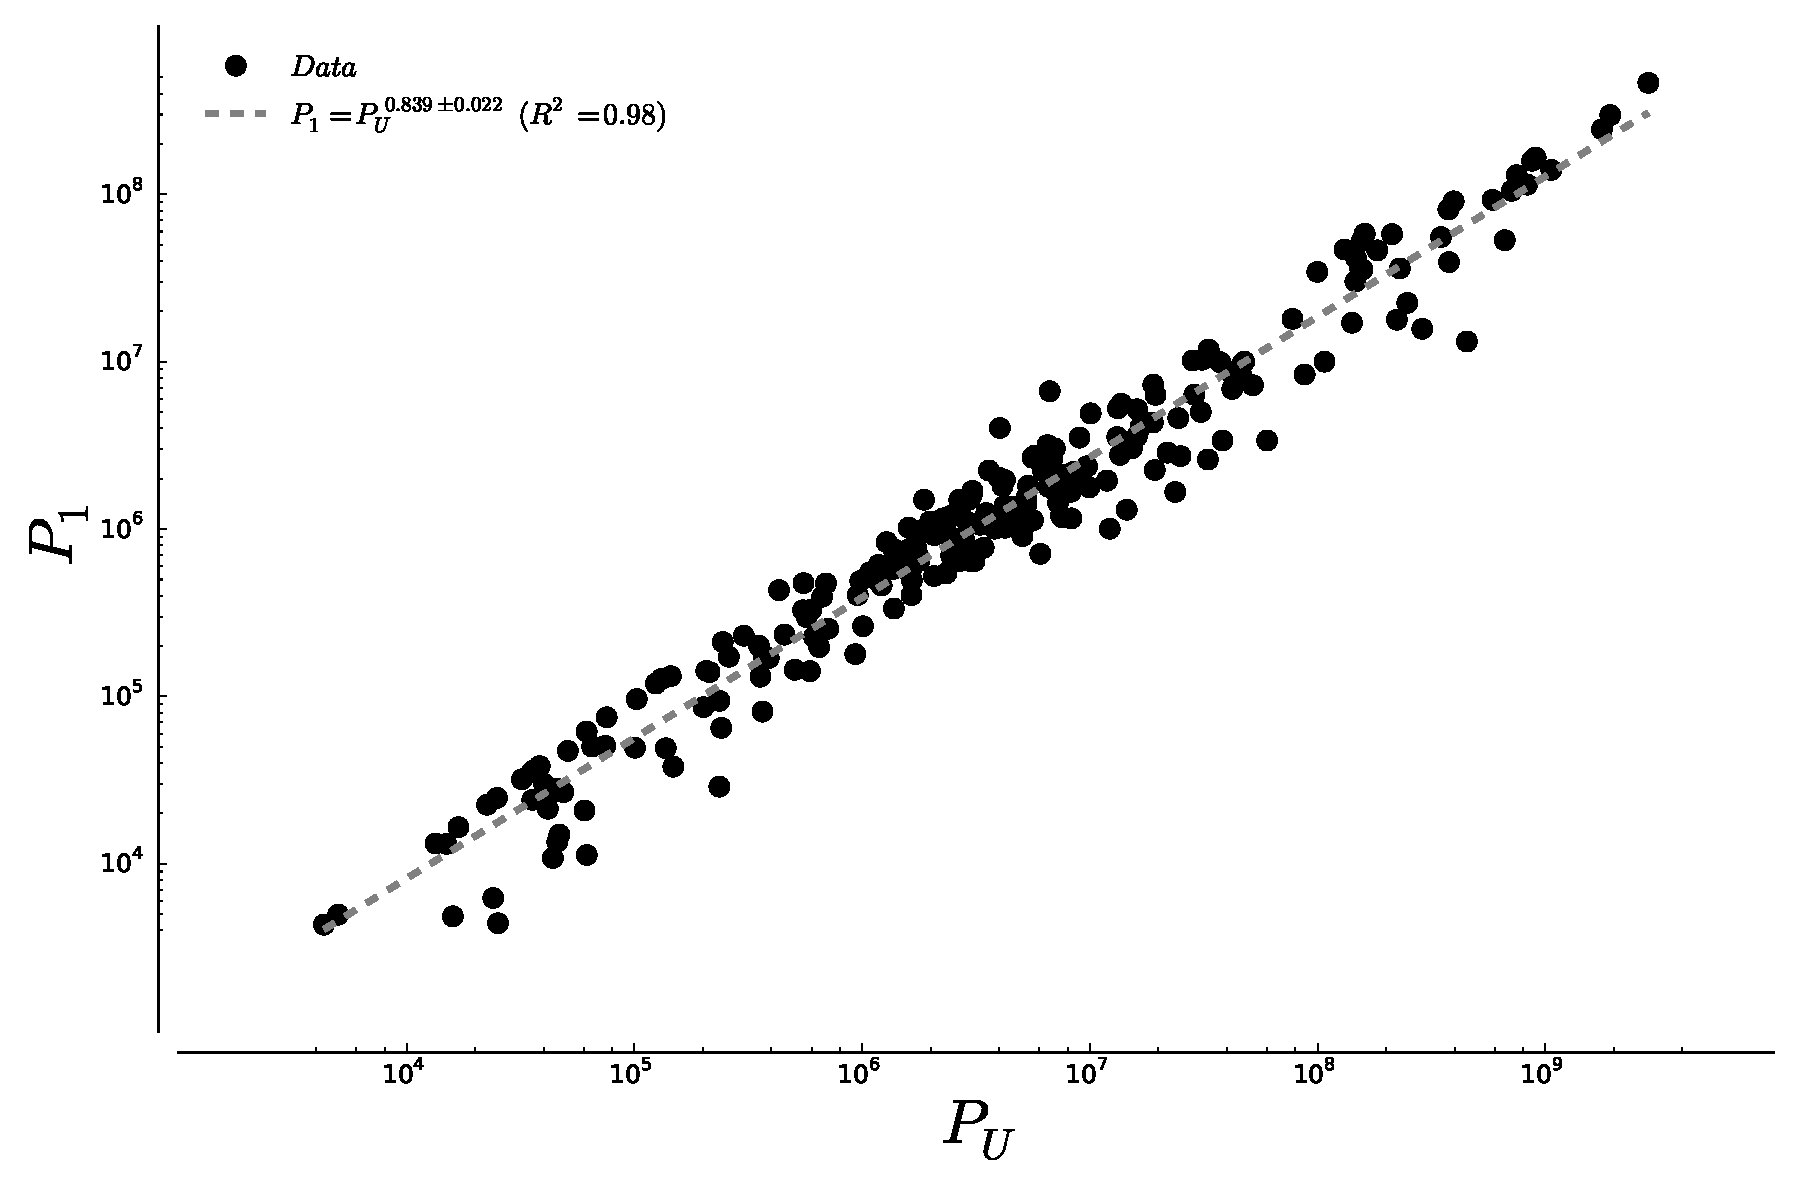
\includegraphics[width=\textwidth]{gfx/chapter-intro/law_metropolises.pdf}
    \caption{{\bf The law of metropolises.} Population of the largest city of
    systems of cities $P_1$ versus the total urban population $P_u$ in that
system. The dashed line shows the result of a powerlaw fit, whose exponent
agrees well with the one found in~\cite{Pumain:1997}. Data for the total urban
population and the population of the largest city of countries in the year
$2000$ were obtained from
the World Bank.\label{fig:metropolises}}
\end{figure}

Assuming a powerlaw relationship between the two quantities, one finds

\begin{equation}
    P_1 \sim P_U^{\,0.84}\:(r^2=0.98)
    \label{eq:metropolis}
\end{equation}

which agrees very well with the empirical data (for all years where data are
available). It is tempting, at first, to consider this as yet-another emprical
regularity exhibited by urban systems, and try to find a coherent interpretation
in geographical terms. However, as we will show, if we assume that the Auerbach-Zipf
law~\cite{Auerbach:1913,Zipf:1949} holds for each system of cities
individually

\begin{enumerate}
    \item We can derive a relation that fits the data as well as
        Eq.~\ref{eq:metropolis};
    \item The relation is not a powerlaw.
\end{enumerate}



\subsection{Deriving the `law of metropolises'}
\label{sub:deriving_the_law_of_metropolises_}

Let us consider a system of cities comprised of $N$ cities, with total
population $P_U$. The size of the largest city is noted $P_1$. We assume that
the distribution of city sizes follows the Auerbach-Zipf law, so that the city
of rank $r$ (the $r$th largest city) has a population

\begin{equation*}
    P_r = P_1\,r^{-\mu}
\end{equation*}

So the total population in the system of cities can be written

\begin{equation}
    P_U = \sum_{r=1}^N P_r = P_1\,\sum_{r=1}^{N} \frac{1}{r^\mu}
\end{equation}

If we assume that $\mu=1$, $P_U$ is given by the harmonic series, and thus

\begin{equation}
    P_U = P_1 \left[ \ln(N) + \gamma + O\left(\frac{1}{N}\right)\right]
\end{equation}

where $\gamma \approx 2.58$ is Euler's constant. This gives us a first relation
between $P_1$, $P_U$ and $N$.\\

Still using the assumption that the distribution of city size follows the
Auerbach-Zipf law with $\mu=1$, we can show (using extremal value
theory)~\cite{Clauset:2009} that on average\graffito{'Average' as in {\bf
ensemble average}} the size of the largest city is proportional to the total
number of cities

\begin{equation*}
    P_1 \propto N
\end{equation*}

Thus, when the number of cities in the system is large, $N \gg 1$ the following
relation holds 

\begin{equation}
    \boxed{P_1\,\ln(P_1) = P_U}
    \label{eq:metropolises_debunked}
\end{equation}

As one can see on Figure\ref{fig:metropolises_debunked}, the formula given by
Eq.~\ref{eq:metropolises_debunked} fit the data as well as the previous one.

\begin{figure}[!h]
    \centering
    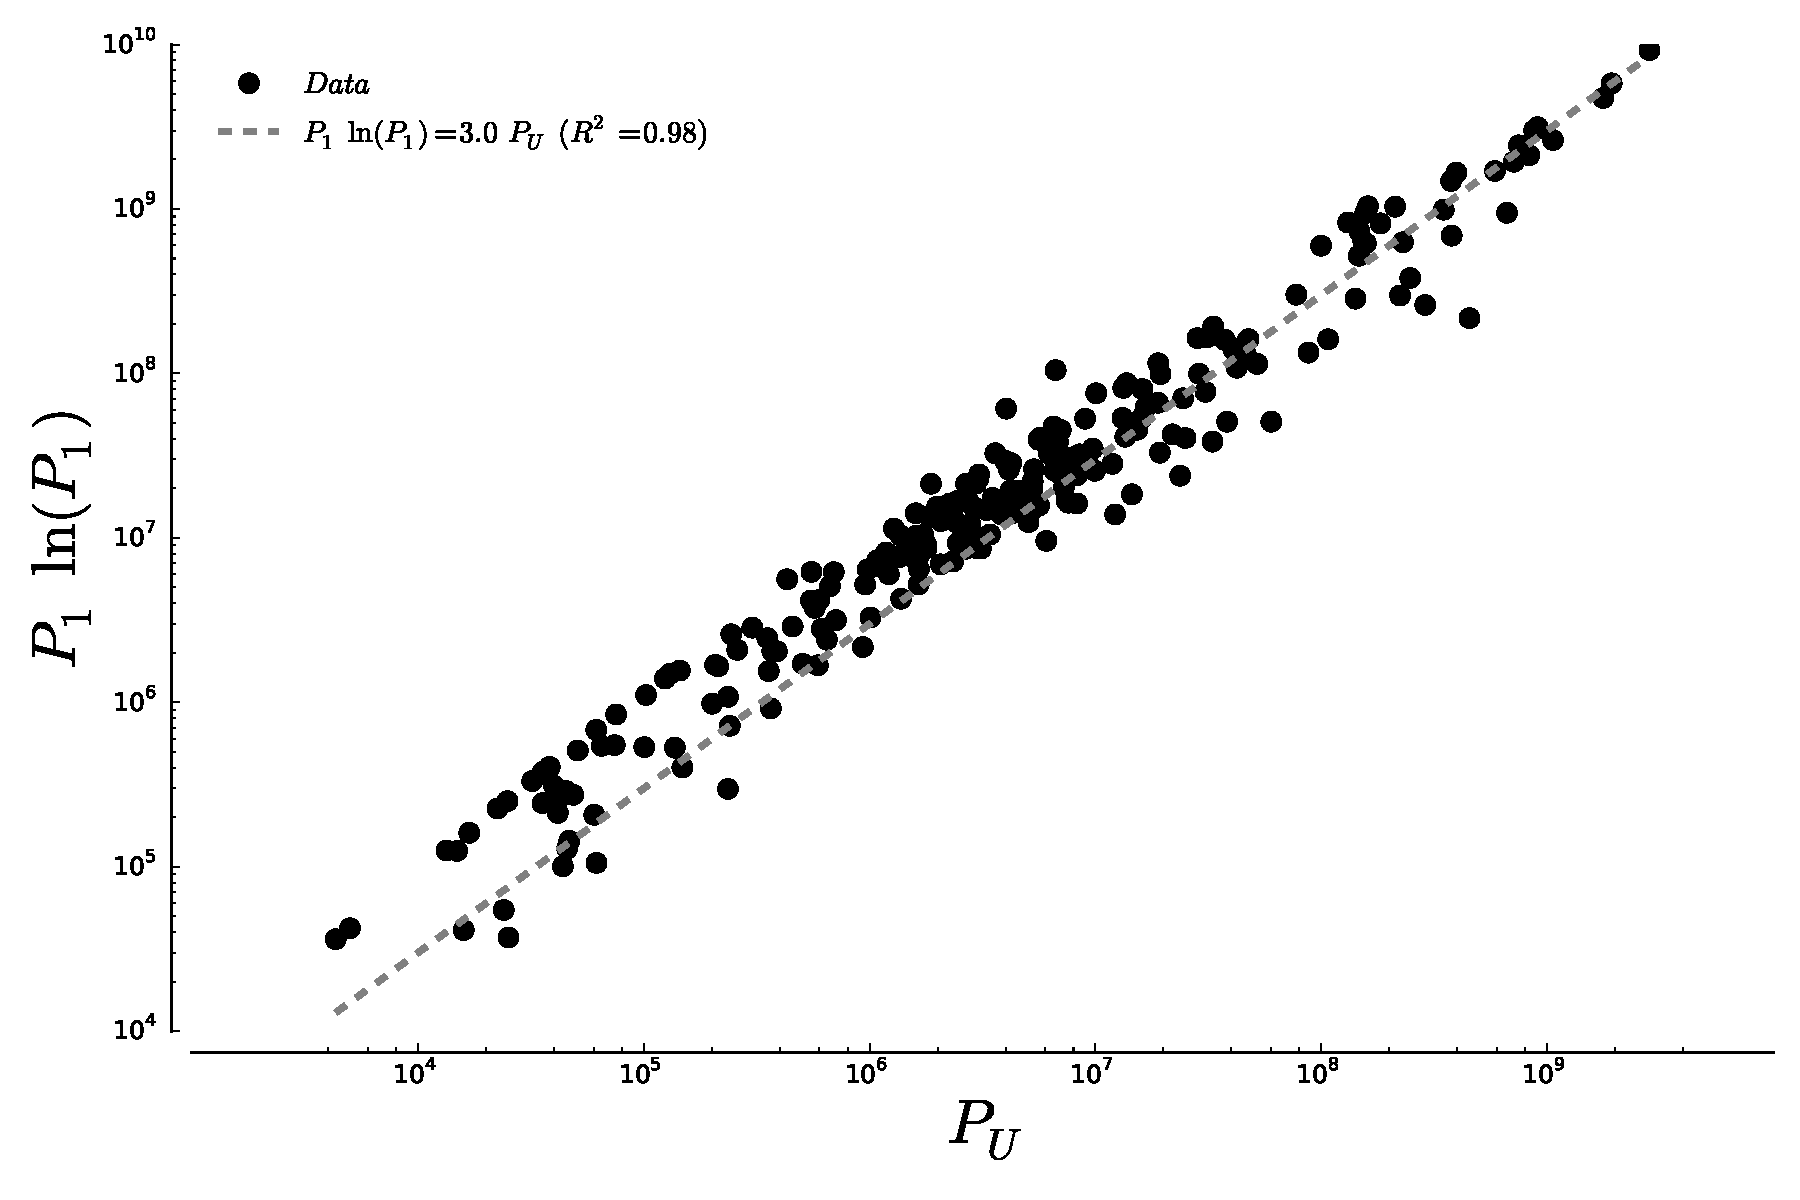
\includegraphics[width=\textwidth]{gfx/chapter-intro/law_metropolises_debunked.pdf}
    \caption{{\bf The law of metropolises revisted.} $P_1 \ln(P_1)$ versus the total urban population $P_u$ in that
system. The dashed line shows the result of a linear fit, which agrees as well
with the data as does the powerlaw relation assumed in~\cite{Pumain:1997}. Data for the total urban
population and the population of the largest city of countries in the year
$2000$ were obtained from
the World Bank.\label{fig:metropolises_debunked}}
\end{figure}


It is therefore impossible to determine which of
Eq.~\ref{eq:metropolises} of Eq.~\ref{eq:metropolises_debunked} describes the
`true' relation between $P_1$ and $P_U$ based on data analysis alone.
Nevertheless, the later finds a very simple explanation in the fact that cities
in systems of cities follow the Zipf-Auerbach law up to a good
approximation. In the absence of any theoretical explanation for the powerlaw
relationship and given the empirical equivalence of both forms, it
least-assuming to consider $P_1 \ln P_1 \sim P_u$.


\subsection{Lessons learned}
\label{sub:lessons_learned}

So, not only is the \emph{law of metropolises} not a fundamental relation, it is
rigorously wrong. 

This teaches us that, given the range of variations of the measured
quantities, it is very difficult to distinguish empirically a powerlaw
relationship from something qualitatively different such as $Y \ln Y \sim P$.
One should therefore be wary of interpreting empirical relationships,
like the one originally found in~\cite{Pumain:1987}, unless a mechanistic
explanation of the fitted relationship is provided. As a matter of fact, what
was thought as a fundamental law might end up being trivial and without great
interest.

We will discuss this matter again in Chapter~\cite{chap:scaling-implications} when
discussing the conclusions we can draw from the analysis of scaling
relationships. But before doing so, we need to talk about models and theories.


\section{Of models and theories}

\subsection{Why bother?}
\label{sub:why_bother_}

As scientific sceptics often like to remind us, all models, all theories are
wrong. But surely, there must be some interest in models to make them deserve
the months, sometimes years of work that scientist devote to them. Admittedly,
many take for granted the usefulness for model, or it seems so obvious that they
never question their quest.

The models two main functions are , broadly speaking, to understand, and to
predict.  The notion of simplification is close to the notion of `mental
economy' defended by the Philosopher of Science Ernst Mach.  According to him,
models' main function is to allow us to condense an infinity of possible
situations in very compact descriptions. Take Snell's law of refraction between
two media of optical indices $n_1$ and $n_2$

\begin{equation}
    n_1\,\sin \theta_1 = n_2\,\sin \theta_2
\end{equation}

In a single formula are contained an infinite number of possible experimental
configurations. Through this model, we are able

This picture is obviously incomplete. Some models obviously do not aim at being
correct from the beginning.

\subsection{Theory, not analogy}
\label{sub:theory_not_analogy}




There are two issues with the current state of affair 
Fancy words are too often used as a substitute for a real
understanding of the system. But, however intellectually appealing they are,
metaphors are not a theory. What do we understand from the comparison of cities
with biological systems? What new knowledge do we gain? Sure, the most important
ideas are those that you trigger, but you are responsible for the way your ideas
are interpreted.  Maybe cities are an easy pray for this sort of behaviour.
Since there is very little understandin, and the immediacy, complexity and
diversity of out experiences with cities creates this big gap in which anyone
can slip an idea or two, that will be interpreted in very different ways by
different people. The genius of metaphors is not to provide interesting ideas
that are ready to be applied to a specific fiedld. Rather, it is to trigger very
different ideas into different people. But this when we should realise the power
of the metaphor and leave it behind, following the trail of the new ideas thus
triggered. What we need to highlight are regularities, not similarities.

What is wrong, and somwehat uncomfortable in the present literature, is the
impression that models and reality live in two distinct, very loosely connected
worlds. Often, the gap is bridged through some intellectual trick, be it analogy
or metaphor.

A very nice quote is the beginning of the EPR paper

In the following manuscript, I will therefore pay a special attention to the
rigour in the language used. Qualify suggestions, by presenting them as such.
This kind of work may be less suggestive, the vocabulary used less expressive,
it may not make the reader feel as good about herself, but it is a necessary
step towards a science of cities. We need to clear the language of unfruitful
metaphors and fill the gap with mechanisms.
